\documentclass[aspectratio=43,english]{beamer}

\usepackage[english]{babel}

\usepackage[T1]{fontenc}
\usepackage[utf8]{inputenc}
\usepackage{lmodern}
\usepackage{pgfplots}
\usepackage{xifthen}
\usepackage{newunicodechar}
\usepackage{textcomp}
\usepackage[absolute,overlay]{textpos}
\usepackage{xparse}

\newunicodechar{°}{\textdegree}
\newunicodechar{µ}{\textmu}

\newcommand*{\ft}{\frametitle{\secname}}
\newcommand*{\ftsub}[1]{\frametitle{\secname\ - #1}}
\newcommand*{\itemp}{\item}
%\newcommand*{\itemp}{\pause\item}
\newcommand*{\+}{\texttt{+}}

\newcommand{\sectionframeimpl}[2]{
	\begin{frame}
	#1
	\begin{itemize}
	#2
	\end{itemize}
	\end{frame}
}
\NewDocumentCommand{\sectionframe}{s m m}{
	\IfBooleanTF{#1} {
		\section*{#2}
	} {
		\section{#2}
	}
	\sectionframeimpl{\ft}{#3}
}
\NewDocumentCommand{\subsectionframe}{s m m}{
	\IfBooleanTF{#1}{
		\subsection*{#2}
	} {
		\subsection{#2}
	}
	\sectionframeimpl{\ftsub{#2}}{#3}
}
\NewDocumentCommand{\subsubsectionframe}{s m m}{
	\IfBooleanTF{#1}{
		\subsubsection*{#2}
	} {
		\subsubsection{#2}
	}
	\sectionframeimpl{\ftsub{#2}}{#3}
}

\beamertemplatenavigationsymbolsempty

\mode<presentation>{
	\usetheme{Madrid}
	\usecolortheme{spruce}
}

\begin{document}

% "I want to give a overview about the Nouveau project and what challenges we deal with reverse engineering Nvidia GPUs. This includes security mechanisms Nvidia added over time to their GPUs to prevent us from doing our job. Having an open source GPU driver is important, because nearly everything somebody does on their Linux driven machine goes through the graphical stack and therefore a lot of sensible information goes through it and why should we trust closed source software with our stuff? Main topics will be which parts of the graphics stack we work on, our goals, what we have achieved already, what tools we are working with to trace the Nvidia driver, how somebody interested in this project can help out, what we currently are working on and what I would like to see implemented next."

% Topics:
% graphic stack parts
% goals
% tools
% current work
% wish list

\title[Nouveau]{Nouveau \\  reverse engineering Nvidia GPUs}
%\author{Karol Herbst}
\date{}

\begin{frame}
\titlepage
\end{frame}

\section*{Overview}

\begin{frame}
	\ft
	\setcounter{tocdepth}{1}
	\tableofcontents
\end{frame}

\sectionframe{Goals}{
	\itemp Understanding the hardware
	\itemp Completely open alternative to closed driver
	\itemp Being able to do research by tweaking
	\itemp To have fun!
}

\section{Reverse Engineering}
\subsectionframe{Hardware}{
	\itemp memory mapped I/O "registers"
	\itemp Engines
	\begin{itemize}
		\itemp PDISP (Display Engine)
		\itemp PGRAPH (Rendering Engine)
		\itemp Video Engines
		\itemp PMU
		\itemp many more
	\end{itemize}
	\itemp ISAs
	\begin{itemize}
		\itemp shaders/CUDA cores
		\itemp fµc
	\end{itemize}
	\itemp GPIO / I²C devices
	\begin{itemize}
		\itemp Sensors
		\itemp Fans
		\itemp Voltage control
		\itemp LEDs
	\end{itemize}
	\itemp Tools: mmiotrace \+ demmio, envydis
}

\subsubsectionframe{Mmiotrace}{
	\itemp In-kernel tracer for MMIO
	\itemp Traces communication between a kernel driver and its devices
	\itemp "abuses" Page faults
	\itemp demmio (enytools) used to parse traces
	\pause\only<2>{
		\begin{textblock*}{0cm}(0.1cm,2.4cm)
			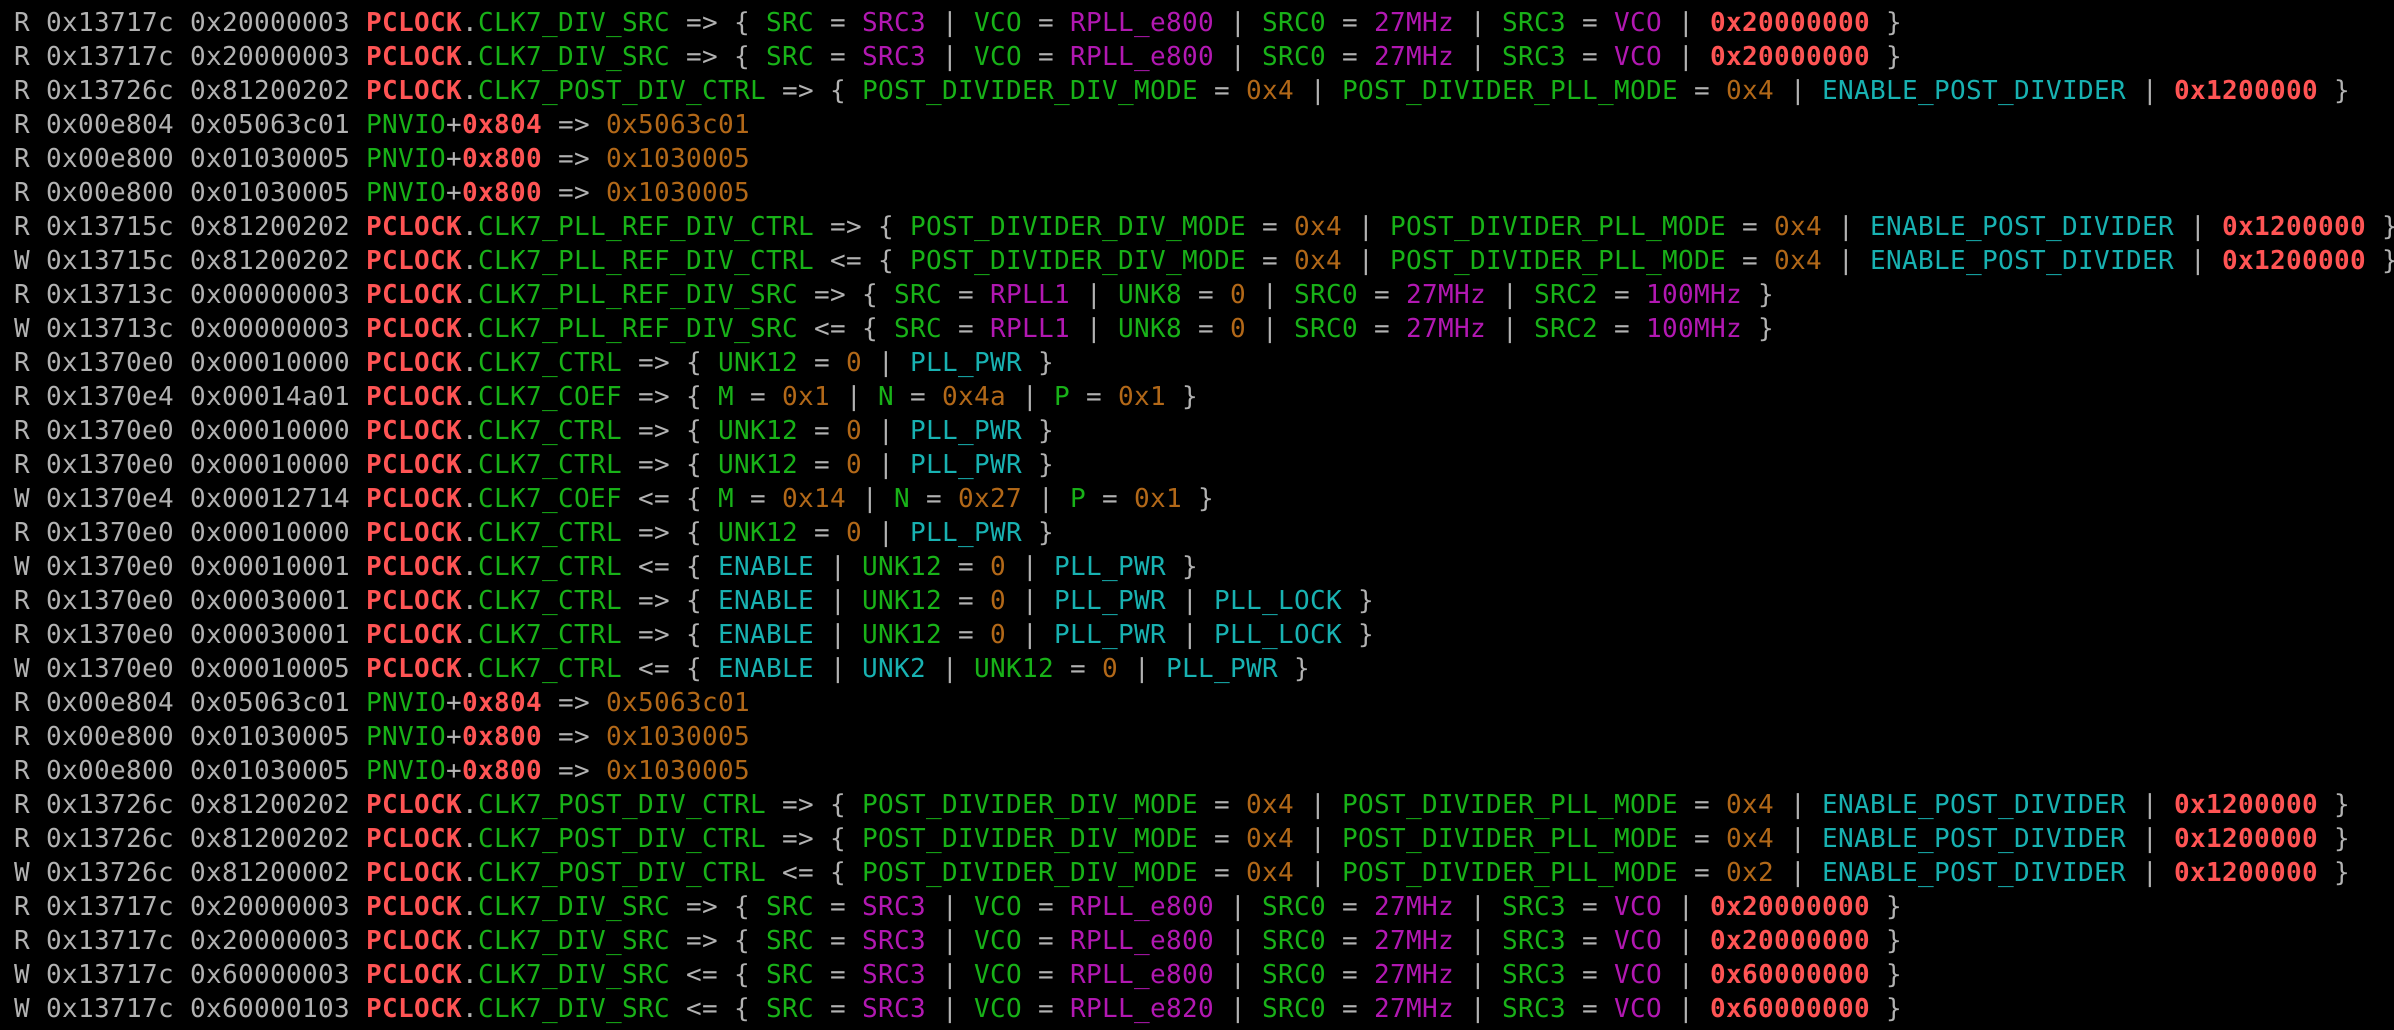
\includegraphics[scale=0.199]{mmiotrace_reclocking}
		\end{textblock*}
	}
}

\sectionframe{Current Challenges}{
	\itemp Pass Khronos CTS for exposing OpenGL 4.4\+
	\itemp Improving Performance
	\itemp Maxwell2\+
	\begin{itemize}
		\itemp Signed VBIOS
		\itemp Signed Firmware
		\begin{itemize}
			\itemp Fan control
			\itemp Reclocking (since Pascal)
			\itemp Tons of other stuff as well (since Pascal)
		\end{itemize}
		\itemp 128 bit AES key
		\itemp Harder REing of VBIOS and MMIO registers
	\end{itemize}
	\itemp Compute support (OpenCL, CUDA)
}

\sectionframe{How to help}{
	\itemp Own hardware with bugs running Nouveau and fix those
	\itemp Be interested and motivated
	\itemp GSoC/EVoC (for students)
}

\end{document}